\chapter{Iterations} \label{ch:iterations}

Iteration objects provide a means of plotting kinematic outputs across a range of kinematic states.  The settings for these plots are stored in .iteration files.

When a new iteration is created, default settings for the iteration are loaded from the configuration file.  These defaults can be configured by the user (see \sref{sec:optionsTab}).

When an iteration file is active, the \element{Main Display Area} contains a rendering of the plot, as configured by the user.  The user can interact with the plot and perform mathematical operations on plotted data.  More information is in \sref{sec:plotDisplay} below.

Also when selected, the Edit Panel will contain three tabs.  These tabs are described in \sref{sec:rangeTab}--\ref{sec:optionsTab} below.

Behavior of the iteration can be further customized by using the options provided in the \element{Iteration} menu, which is described in \sref{sec:iterationMenu}.

\section{Plot Display} \label{sec:plotDisplay}

The plot is displayed in the \element{Main Display Area}.  Below the plot is a list of all of the active plots.  Here, curves can be toggled on/off or optionally plotted against the right y-axis instead of the left.  The color, size and marker size for each curve can be independently adjusted.  Right-clicking on the plot area or the plot list will generate a context-sensitive pop-up menu.  These pop-up menus provide a means of performing mathematical operations on plotted data, fitting curves to plotted data, changing plot background colors, toggling the legend on or off and more.  The legend can be dragged and dropped to place it in the plot area as desired.  Double-clicking in the plot area introduces a cursor, which can be dragged across the extents of the plot area.  The values corresponding to places where the cursor crosses the plot curves are displayed in the grid below the plot area.

An example of an iteration plot is shown in \figref{fig:iteration}.

\begin{figure}
  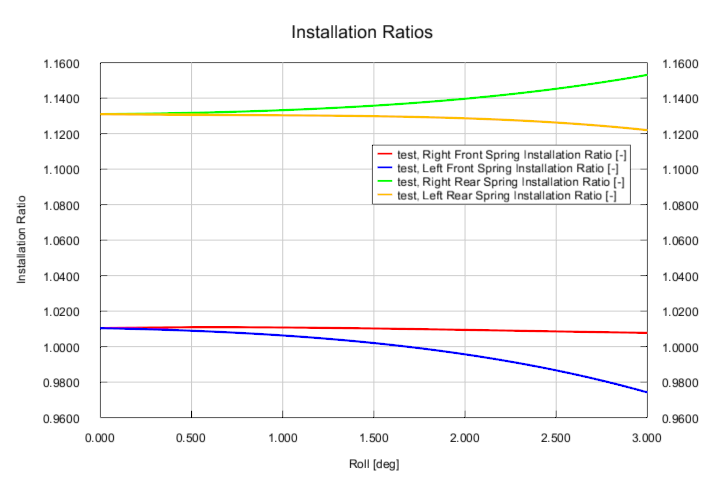
\includegraphics[width=\textwidth]{images/iteration}
  \caption{Example iteration Plot Display showing the installation ratios at all four corners of a vehicle while experiencing roll} \label{fig:iteration}
  \centering
\end{figure}

\section{Range Tab} \label{sec:rangeTab}

The \element{Range} tab describes the range of kinematic states which are to be represented on the plot.  Any combination of pitch, roll, heave and steer can be used as start and end conditions.  The number of points used on the plot can also be adjusted.  Generally, kinematic outputs change slowly and smoothly with respect to the kinematic states.  For these cases, smooth curves can be produced with a relatively few number of points.  Occasionally, however, an output will appear to change rapidly and more points are required to produce a smooth curve.  It is advisable to use as few points as possible, especially if the iteration is to be associated with several open car files, as each additional point requires another sequence of calculations for each associated car.

Note that when the range of kinematic outputs includes changes in more than one parameter simultaneously, the curves in the resulting 2D plot can be thought of as a diagonal slice through the output surface.  In other words, moving along a plot curve means all varied kinematic inputs are changing --- the independent variable is actually a combination of varying kinematic inputs.

\section{Active Plots Tab} \label{sec:activePlotsTab}

The \element{Active Plots} tab allows the user to specify which outputs should be plotted in the active iteration file.  It is possible to select as many outputs for plotting as desired.

\section{Options Tab} \label{sec:optionsTab}

The \element{Options} tab allows the user to manually specify the plot title and axis labels.  There is also an option that permits toggling the grid lines on and off.

At the bottom of the panel is a button labeled \button{Set As Default Properties}.  Clicking this button will save all of the current plot configuration options to the configuration file.  Each time a new iteration file is created, this configuration will be applied.

\section{Iteration Menu} \label{sec:iterationMenu}

All iteration data is exportable into a .csv format which can be opened with Microsoft Excel or other tools.  This can be done by selecting the \button{Export Data} entry in the \element{Iteration} Menu.

By default, iterations auto-associate with all open car files.  This means that the desired kinematic outputs are plotted for every open car.  This makes side-by-side comparisons of different geometries easy.  If this is not desired, the \button{Associated Cars} entry in the \element{Iteration} menu can be used to specify which cars should be analyzed by the iteration file.

\vvase{} will automatically select the correct independent variable for the plot when only a single kinematic input is varied.  For cases when multiple kinematic inputs are varied, the user can select the independent variable by selecting the \element{Set X-Axis} entry in the \element{Iteration} menu.
